\documentclass[12pt]{article}
\usepackage[a4paper, bindingoffset=0.2in, %
							left=0.5in,right=0.5in,top=0.5in,bottom=0.5in,%
							footskip=.25in]{geometry}
\usepackage{graphicx}
\usepackage{listings}
\usepackage{amssymb}
\usepackage{amsmath}
\usepackage{hyperref}


\title{PSet3 Report}
\author{Ali Abolhassanzadeh Mahani}

\begin{document}
	\maketitle
	\section{Standard Deviation}
	\section{Random Walk}
	I made a function \texttt{rw\_next()} that takes the current postion and moves to left / right 
	with a given probability.
	Then I simulate the random walk and take the data. I took the data in 100 choice intervals, from
	100 to 1000 and ran the simulation 10000 times in the \texttt{rw\_simul()} function.
	The plots are available in Fig\ref{fig:rw_sim})
	\begin{figure}[h!]
		\centering
		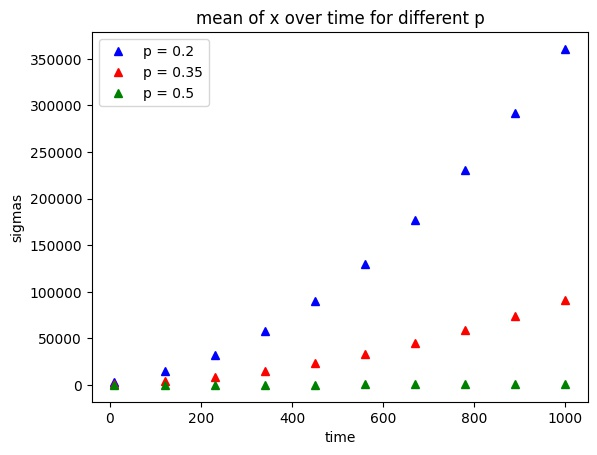
\includegraphics[width=0.9\linewidth]{../p2/sigmas.jpg}
		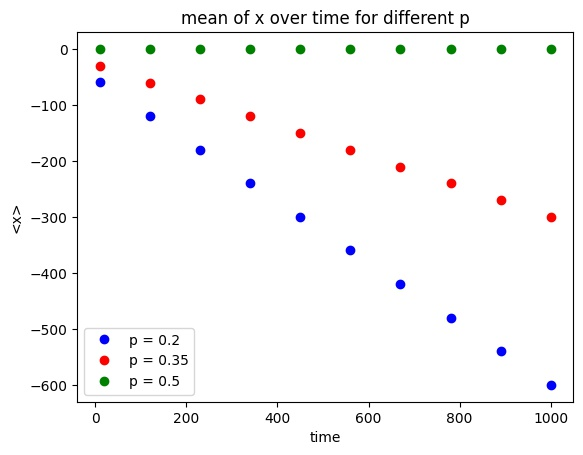
\includegraphics[width=0.9\linewidth]{../p2/x_means.jpg}
		\label{fig:rw_sim}
		\caption{The plot of $\sigma^2$ (top) and $<x>$ (bottom) over time for different probabilities. Took 10000 runs and got the mean.}
	\end{figure} 

	\section{Random Walk with Trap}
	I simulated this problem using a class called \texttt{Drunk}. This is the actualization of a 
	drunk person dangling around in 1-D. I set the path to be from 0 to 19 and traps at -1 and 20.
	If the drunk gets to those points, it perishes and I can then get its lifetime.
	I ran the simulation for 10000 drunk men and took the mean.
	The resulting graph is plotted in Fig\ref{fig:rw_trap}
	\begin{figure}[h!]
		\centering
		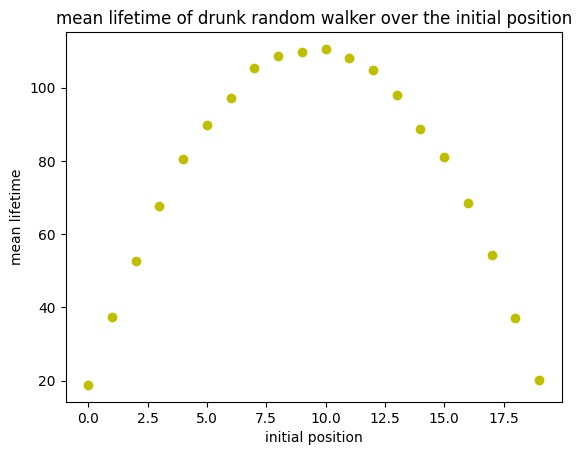
\includegraphics[width=0.9\linewidth]{../p3/drunk.jpg}
		\label{fig:rw_trap}
		\caption{mean lifetime over different indices of the path. traps at -1 and 19. Ran 10000
		instance simulations}
	\end{figure}

	\section{2-D Random Walk}
	This time, I simulated the \texttt{Drunk} person to be a girl on a 2-D surface. Almost the same as the 1-D instance, but returns $r^2$. I ran the simulation with time intervals of 100 for 10 intervals. The plot is available in Fig\ref{fig:2d_rw}
	\begin{figure}[h!]
		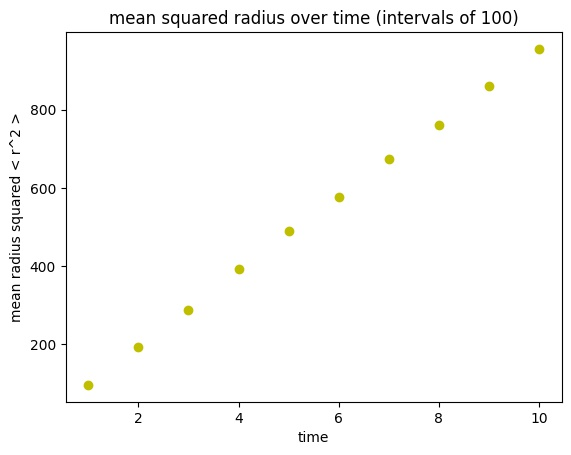
\includegraphics[width=0.9\linewidth]{../p5/2d_girl.jpg}
		\label{fig:2d_rw}
		\caption{dependence of The distance squared $r^2$ over time intervals of 100 choices.}
	\end{figure}
	
	\section{Aggressive Layer Deposition}
	I made a \texttt{RandWalker} class that generates a particle at a random x and the highest y
	that I chose to be 199. The length of the seed is 201 for symmetry that proved to play no role
	in the simulation whatsoever :-) \\
	I chose the buffer length to be 10. If the particle exceeds that buffer, I reset the position with
	a random $x$ position again.
	
	I made 2000 particles and gave them room to random walk and stick to the seed. Then I 
	visualized the grid using \texttt{plt.pcolor()}.
	
	I also tried changing colors but apparently something is wrong with it. Maybe the color code intervals.
	
	The plot is in Fig\ref{fig:ald}
	\begin{figure}[h!]
		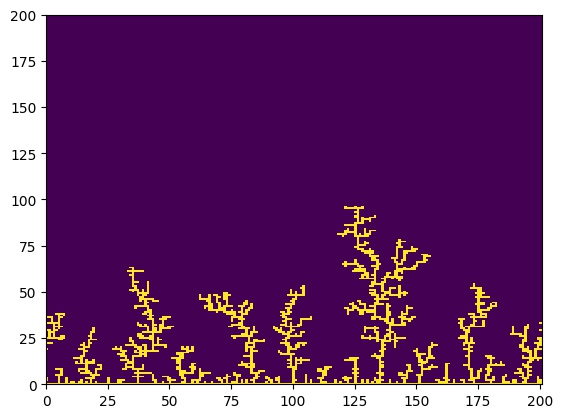
\includegraphics[width=0.9\linewidth]{../p6/ald.jpg}
		\label{fig:ald}
		\caption{deposited 2000 randomly positioned particles using random walk simulation.}
	\end{figure}
\end{document}